%!TEX root = ../main.tex

\graphicspath{{./figures/chapter5/}}

\chapter{Transcript localization}
\label{ch:chapter5}

\minitoc
\newpage

In this chapter we present several applications of the pipeline described in the previous chapters.
More specifically, we analyze experimental datasets in order to explore, quantify and validate biological insights about \ac{mRNA} localization.
Results from this chapter are computed from three different high content screening studies, totaling tens of transcripts observed through thousands of bioimages.

In the first section, we develop a general classification pipeline to identify generic \ac{mRNA} localization patterns from \ac{smFISH} images~\cite{CHOUAIB_2020}.
In the second section, exploiting the same dataset, we focus on a specific and novel clustering pattern: the translation factories.
These first two sections describe the work published in:

\begin{center}
	\color{green}
	R. Chouaib, A. Safieddine, et al. (2020), \textit{A dual protein-mRNA localization screen reveals compartmentalized translation and widespread co-translational RNA targeting}, Developmental Cell 54 (6), 773.
\end{center}

In the third section, we exploit a \ac{GFP} channel to visualize and detect centrosomes.
We observed a centrosomal localization patterns for different transcripts and different mitosis phases~\cite{safieddine_choreography_2021}.
This work was published in:

\begin{center}
	\color{green}
	A. Safieddine, E. Coleno, et al. (2021), \textit{A choreography of centrosomal mRNAs reveals a conserved localization mechanism involving active polysome transport}, Nature Communications 12 (1), 1352.
\end{center}

In the fourth section, we detail several transcripts with a protrusion localization pattern~\cite{pichon_kinesin_2021}.
This last section mainly describes results presented in:

\begin{center}
	\color{green}
	X. Pichon, K. Moissoglu, et al. (2021), \textit{The kinesin KIF1C transports APC-dependent mRNAs to cell protrusions}, RNA 27 (12), 1528.
\end{center}

\section{General pattern recognition}
\label{sec:general_pattern_recognition}

Our first large-scale application of the pipeline described in the previous chapters consists in classifying individual cells with one or several \ac{RNA} localization patterns.
This work is published in~\cite{CHOUAIB_2020}.

\subsection{Introduction}
\label{subsec:introduction_general_pattern}

\begin{center}
	\textit{(To be completed)}
\end{center}

% paper FQ2

% In Chouaib et al. (2020), we performed a high-content screen in HeLa cells and analyzed 10,000 segmented cells.
% FISH-quant v2 was used for spot detection, cell segmenta- tion and the computation of localization features
% that al- lowed us to apply supervised and unsupervised machine learning to identify localization patterns and
% classify single cells into predefined pattern classes. We observed several distinct mRNA localization patterns,
% including RNA accu- mulating (i) in foci, (ii) in cytoplasmic protrusions, (iii) in the perinuclear area
% (which could be subdivided in endo- somal, RE, Golgi and centrosome associate), (iv) forming a rim at the nuclear edge, or (v) inside the nucleus (Fig. 2).
% Interestingly, automated classification done on a single-cell level revealed a high degree of
% cell-to-cell het- erogeneity in RNA localization, with 10% to 80% of the cells displaying the
% expected pattern depending on the RNA (Fig. 5A). In addition, for each pattern, only a fraction of
% the mRNA appeared to localize, revealing a high degree of plasticity in RNA localization mechanisms.
% This appears to be specific to cell lines as RNA localization in embryos is usually much more stereotyped.
% We also quantified how translation inhibition affected RNA localization and found that most mRNAs localize in a
% translation-dependent man- ner, which is unexpected (Fig. 5B). This also enabled us to discover translation factories,
% small cytoplasmic structures where specific mRNAs accumulate to be translated.

\subsection{Materials and methods}
\label{subsec:materials_general_pattern}

The quantitative pipeline used in this study and the existing work in FISH-quant V1 are the building blocks of FISH-quant V2.
Therefore, the various methods presented here were not yet packaged in \emph{bigfish}, but Python packages that formed its foundation are already in used.
This work is developed in Python and the code repository is public\footnote{\url{https://github.com/Henley13/paper_translation_factories_2020}}.

\subsubsection{Experimental data}

At first more than 500 genes have been manually analyzed to identify potential transcripts with non random localization patterns within the cell.
In addition to different qualitative and manual observations performed over this dual \ac{RNA}-protein localization screen, we also develop a quantitative pipeline to systematically classify transcripts' localization patterns.
To this end, I exploit a dataset of 526 \ac{FoV}s, combining DAPI and \ac{smFISH} channels as illustrated in Figure~\ref{fig:fov_racha}.
The raw images stacks several 2D acquisitions to gather a 3D information of the \ac{FoV} with a z-spacing of 0.3μm.
Acquisitions are performed with a Zeiss Axioimager Z1 widefield microscope or a Nikon Ti fluorescence microscope, on human cell lines HeLa.
In total, this dataset is built from 57 independent experiments gathering observations from 27 different \ac{mRNA}s under different experimental conditions.

\begin{figure}[h]
    \centering
    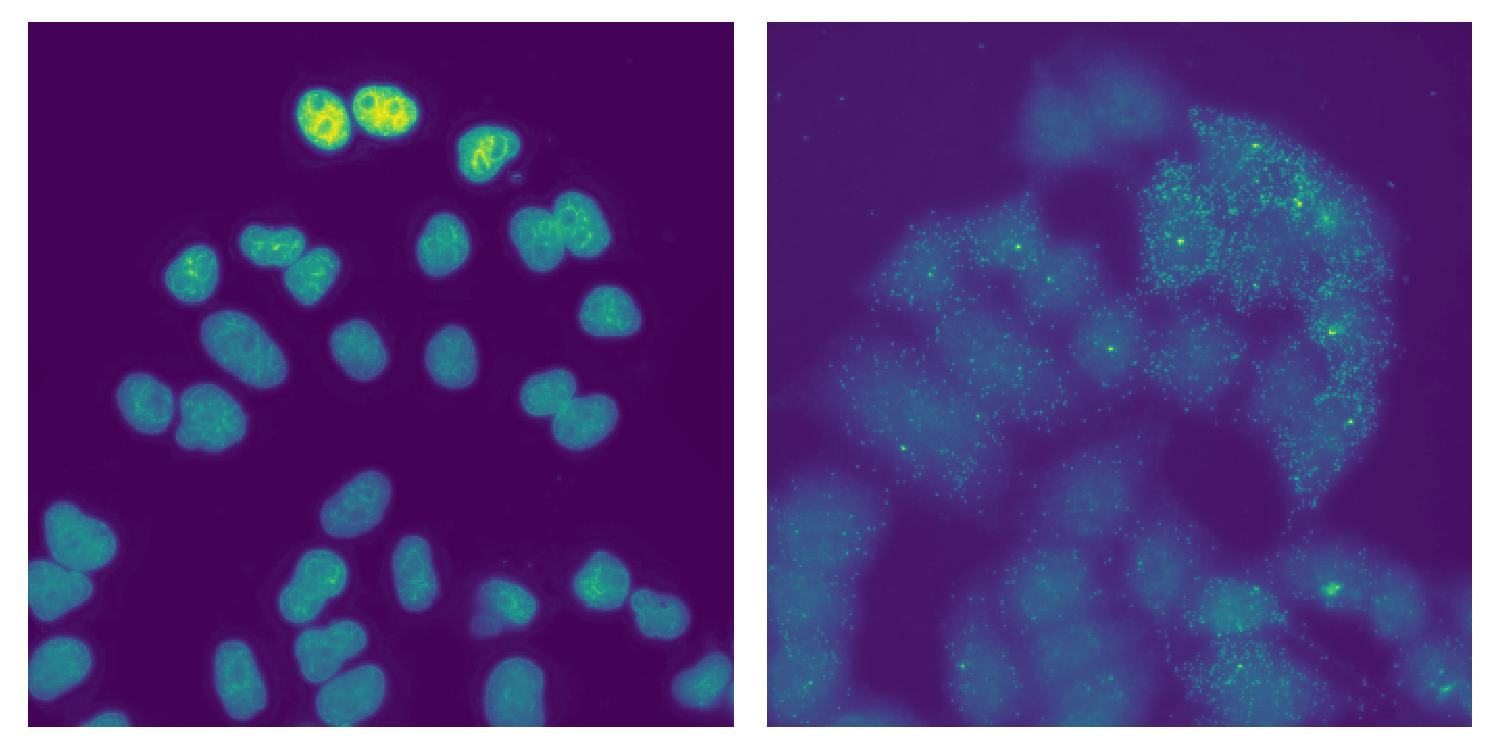
\includegraphics[width=\textwidth]{figures/chapter5/FoV_DYNLL2}
    \caption{Contrasted image with Dapi (\textit{left}) and smFISH (\textit{right}) channels.
	Images are projected in 2D.
	Targeted transcript is DYNLL2.
	Plot build with \emph{bigfish}}
    \label{fig:fov_racha}
\end{figure}

\subsubsection{Semi-automated RNA detection}

\ac{RNA} detection is performed with a Python implementation of FISH-quant v1~\cite{mueller_fish-quant_2013}.
I apply a \ac{LoG} filter on the 3D \ac{smFISH} images, then a local maximum detection algorithm.
However, a threshold value has to be set manually for every experiment to discriminate the actual spots from the noisy background blobs.
Large agglomeration of spots are decomposed with a gaussian mixture model, following~\cite{samacoits_computational_2018}.
Ultimately, \ac{RNA} clusters - namely foci - are detected with a DBSCAN algorithm~\cite{ester_density-based_1996} applied on the detected spots.
According to the way a DBSCAN cluster samples, a foci is then defined as a set of at least 5 points where for each point there is at least one other point from the foci within a 350 nanometers distance.
All foci overlapping the nuclear area in the projected 2D images are considered as a transcription site and removed from the analysis.
Percentages of \ac{RNA} in foci are then calculated as number of \ac{RNA} inside the cytoplasmic foci divided by the number of cytoplasmic \ac{RNA}s.

There are two main differences compared to the current detection methods implemented in FISH-quant and presented in Chapter~\ref{ch:chapter2}: a detection threshold has to be set manually and the decomposition of agglomerated spots has since been simplified.

\subsubsection{Cell and nucleus segmentation}

Nucleus segmentation is performed from the DAPI channel and cell segmentation from the cell autofluorescence in the \ac{smFISH} channel.
Segmentation is performed in 2D for both nuclei and cells, thus 3D images are projected in two dimensions using their maximal local focus values~\cite{tsanov_smifish_2016}.

Nuclei are segmented with NucleAIzer~\cite{hollandi_nucleaizer_2020}, a deep neural network pipeline trained with the annotations from the Data Science Bowl 2018 challenge\footnote{\url{https://www.kaggle.com/c/data-science-bowl-2018}}.
This pipeline is based on a Mask R-CNN architecture~\cite{He_2017_ICCV}, with optionally a fine-tuning of the segmented boundaries with a U-Net model~\cite{Ronneberger_unet}.
After a first round of segmentation, some nuclei are missing, so I remove the segmented nuclei from the DAPI channel and feed NucleAIzer with the remaining nuclei for a second round of segmentation.
Removing the segmented nuclei from the original image implies some morphological mathematics techniques as described in Chapter~\ref{ch:chapter3}.
This technique is now implemented in FISH-quant.

Cells are segmented with a watershed algorithm using nuclei masks as seeds.
A threshold value is set manually for every experiment to discriminate the cell surface from the background.
In case of poor results, some segmentation masks are corrected manually.
This is especially the case for transcript that tend to localize in cell protrusion.
Indeed, such localization pattern is highly sensitive to the segmentation accuracy.

\subsubsection{Binary classification models}

Based on the segmentation masks and the coordinates of the detected spots, I identify 9,710 individual cells with an average of 346 \ac{RNA}s per cell.
For each cell, I collect the cell and nucleus masks in 2D, the \ac{RNA} and the potential clusters coordinates in 3D.
In addition I save an image of the cell, for visualization purpose, and different information about the experiment (the presence of a treatment, the targeted gene, etc.).
Cropped cells, empty cells or cells with less than 30 \ac{RNA} detected inside are removed.
At this point, I have a coordinate representation of every cell, as presented in Chapter~\ref{ch:chapter4}.

I design and compute a set of 15 features to describe the spatial distribution of points inside the cell:
\begin{itemize}
	\setlength\itemsep{0.1em}
	\item The number of foci.
	\item The proportion of \ac{RNA} inside foci.
	\item The proportion of \ac{RNA} inside the nucleus.
	\item The average \ac{RNA} distance to the cell membrane, normalized by the value obtained under a uniform \ac{RNA} distribution.
	\item The average \ac{RNA} distance to the nucleus membrane, normalized by the value obtained under a uniform \ac{RNA} distribution.
	\item The average foci distance to the cell membrane, normalized by the value obtained under a uniform foci distribution.
	\item The average foci distance to the nucleus membrane, normalized by the value obtained under a uniform foci distribution.
	\item The proportion of \ac{RNA} inside cell protrusion.
	A protrusion region is defined by calculating the difference between the segmented cellular region and its morphological opening with a large window.
	\item The peripheral dispersion index, defined as the squared point distance to the centroid of the cell and normalized by the value obtained under a uniform \ac{RNA} distribution.
	\item The number of \ac{RNA}s within 515 nm from the nucleus membrane, normalized by the value obtained under a uniform \ac{RNA} distribution.
	\item The number of \ac{RNA}s between 515 nm and 1030 nm from the nucleus membrane, normalized by the value obtained under a uniform \ac{RNA} distribution.
	\item The number of \ac{RNA}s between 1030 nm and 1545 nm from the nucleus membrane, normalized by the value obtained under a uniform \ac{RNA} distribution.
	\item The number of \ac{RNA}s between 0 nm and 515 nm from the cell membrane, normalized by the value obtained under a uniform \ac{RNA} distribution.
	\item The number of \ac{RNA}s between 515 nm and 1030 nm from the cell membrane, normalized by the value obtained under a uniform \ac{RNA} distribution.
	\item The number of \ac{RNA}s between 1030 nm and 1545 nm from the cell membrane, normalized by the value obtained under a uniform \ac{RNA} distribution.
\end{itemize}

\begin{figure}[h]
	\centering
	\minipage{0.2\textwidth}
		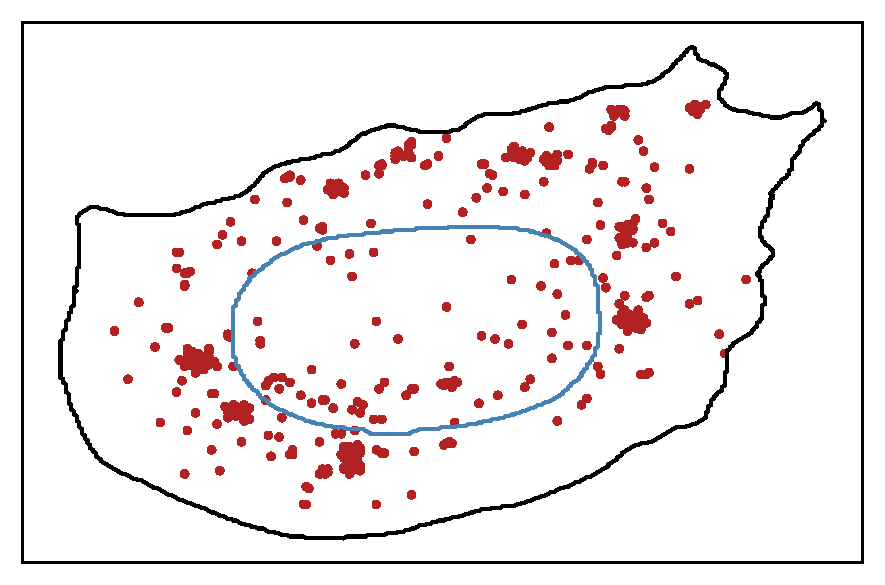
\includegraphics[trim={0.5cm 0.5cm 0.5cm 0.5cm},clip,width=\linewidth]{figures/chapter5/plot_foci}
		\subcaption{Foci}
	\endminipage\hfill
	\minipage{0.2\textwidth}
		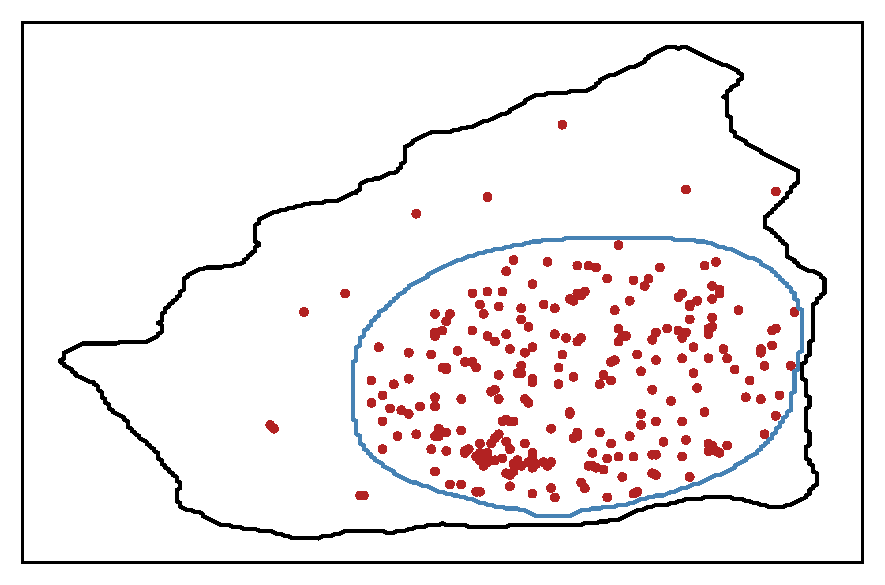
\includegraphics[trim={0.5cm 0.5cm 0.5cm 0.5cm},clip,width=\linewidth]{figures/chapter5/plot_intranuclear}
		\subcaption{Intranuclear}
	\endminipage\hfill
	\minipage{0.2\textwidth}
		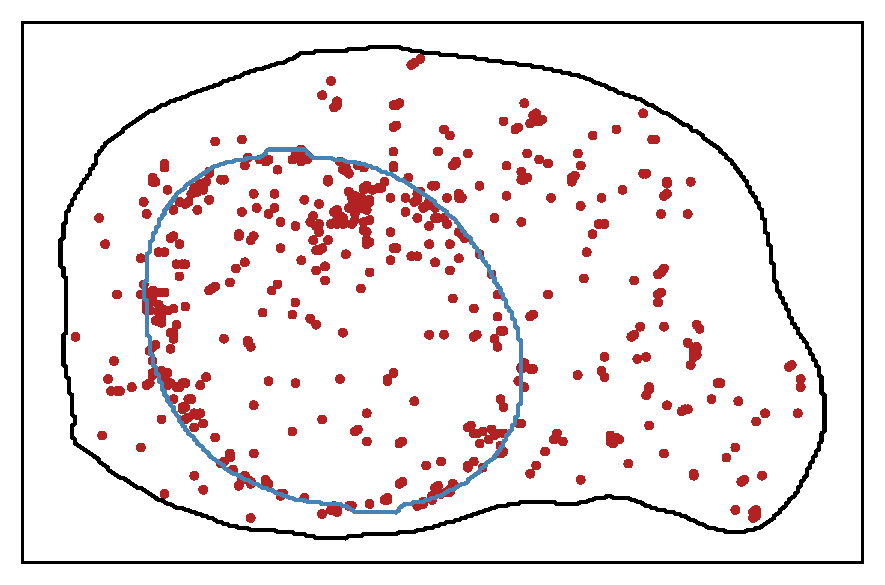
\includegraphics[trim={0.5cm 0.5cm 0.5cm 0.5cm},clip,width=\linewidth]{figures/chapter5/plot_nuclear}
		\subcaption{Nuclear edge}
	\endminipage\hfill
	\minipage{0.2\textwidth}
		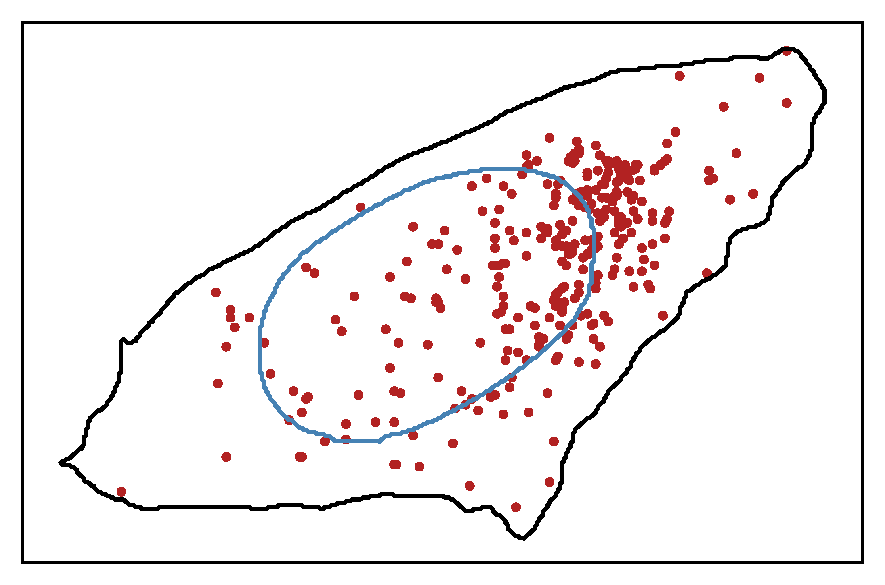
\includegraphics[trim={0.5cm 0.5cm 0.5cm 0.5cm},clip,width=\linewidth]{figures/chapter5/plot_perinuclear}
		\subcaption{Perinuclear}
	\endminipage\hfill
	\minipage{0.2\textwidth}
		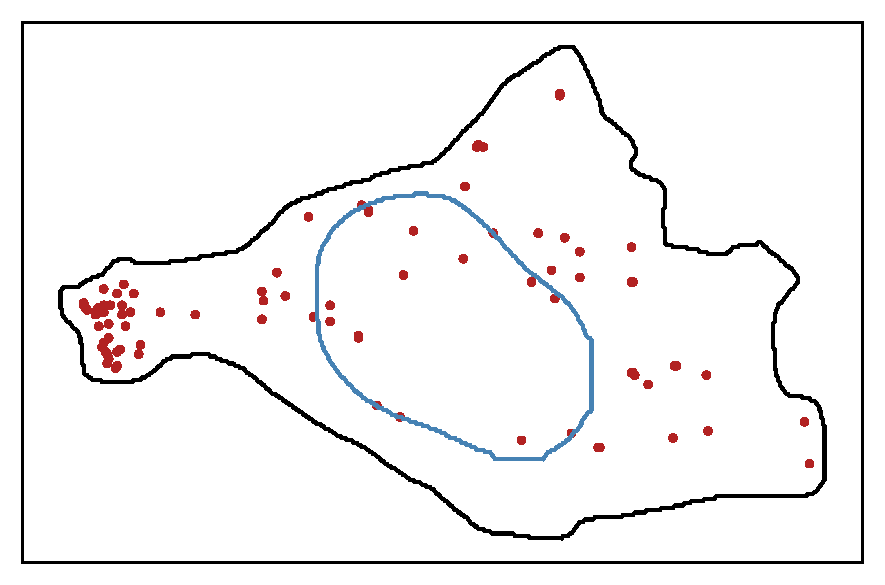
\includegraphics[trim={0.5cm 0.5cm 0.5cm 0.5cm},clip,width=\linewidth]{figures/chapter5/plot_protrusion}
		\subcaption{Protrusion}
	\endminipage
	\caption{RNA localization patterns from~\cite{CHOUAIB_2020}.
	Coordinate representations with RNA spots (\textit{red}), cell membrane (\textit{black}) and nuclear membrane (\textit{blue}).
	Detection and segmentation results are extracted and visualized with \emph{bigfish}}
	\label{fig:localization_patterns_racha_features}
\end{figure}

The apparent precision of the nanometer distances is just an artifact as the concentric regions are delimited visually from a sample of cell images.
Therefore, the width of these regions are defined in pixels, more precisely, with a 5 pixels width and a pixel size of 103 nm.
I use these hand-crafted features to train several binary classifiers, one for each localization pattern we want to recognize.
Five specific localization patterns are defined - foci, intranuclear, nuclear edge, perinuclear, protrusion - and the random pattern is considered as a default one.
Figure~\ref{fig:localization_patterns_racha_features} illustrates an example of these patterns with a coordinate representation.

To train the classifiers, manual annotations are needed as a ground truth.
I generate panels with the cropped original image of the individual cells and their coordinate representations.
These panels are then manually tag with the appropriate localization pattern.
The manual classification result has been independently checked by several trained microscopists.
Ultimately, I end up with 810 annotated cells.
Counts of the annotations are presented in Table~\ref{table:real_dataset_chapter5}.

\begin{wraptable}{L}{0.50\textwidth}
	\centering
	\begin{tabular}{| c | c |}
		\hline
		Pattern & \# of cells \\
		\hline
		Random & 372\\
		Foci & 198\\
		Intranuclear & 73\\
		Nuclear edge & 87\\
		Perinuclear & 64\\
		Protrusion & 83\\
		\hline
	\end{tabular}
	\caption{Annotated cells}
	\label{table:real_dataset_chapter5}
\end{wraptable}

One way to evaluate how relevant is the feature space is to investigate the distribution of the annotated cells within it.
To do so, I reduce the dimensionality with a \ac{t-SNE} transformation~\cite{vandermaaten_2008} in order to visualize the features point cloud.
From the multi-dimensional feature space, I obtain a 2D vector representation I can plot.
In term of setting, I initialize the \ac{t-SNE} with a PCA transformation first and use a perplexity value of 30.

I also define a supervised learning problem with the training of 5 independent binary Random Forest classifiers~\cite{breiman_random_2001}.
The choice to design the problem as several binary ones instead of one multi-class problem allows me to define the localization patterns as non mutually exclusives.
Indeed, an individual cell can display several patterns at the same time, like \ac{RNA} clusters (foci) localizing around the nuclear membrane (nuclear edge).
For each model, I build a training set including all the cells of one class and a subsampling of cells from others classes, such that the imbalance is 1:4 for the positive class.
This is a ''one vs.\ all'' training strategy.
Eventually, I exploit the \ac{OOB} error allowed by the random forest design.
In such manner, the model can ''be fit in one sequence, with cross-validation being performed along the way.''~\cite{hastie_elements_2009}.
Random forest is an ensemble model of tree classifiers.
Each tree is trained on a subsample of the observations and a subset of features.
This ensembling framework makes random forest quite robust to overfitting.
For every sample, an \ac{OOB} prediction can be computed using only the trees fitted without the sample.
I initialize the random forests with 100 trees, a maximal depth of 3 and a minimum number of samples per splitter node of 2.
During the training, for each split, I consider a subset of 10 features and entropy criterion.
In addition, input dataset is rescaled to have zero mean and unit variance.

\subsection{Results}
\label{subsec:results_general_pattern}

Thanks to their design or their normalization, the spatial features selected are mostly invariant to \ac{RNA} concentration.
They allow the use of unsupervised or supervised methods to classify cells among several localization patterns.

\subsubsection{Unsupervised visualization}

\begin{figure}[h]
    \centering
    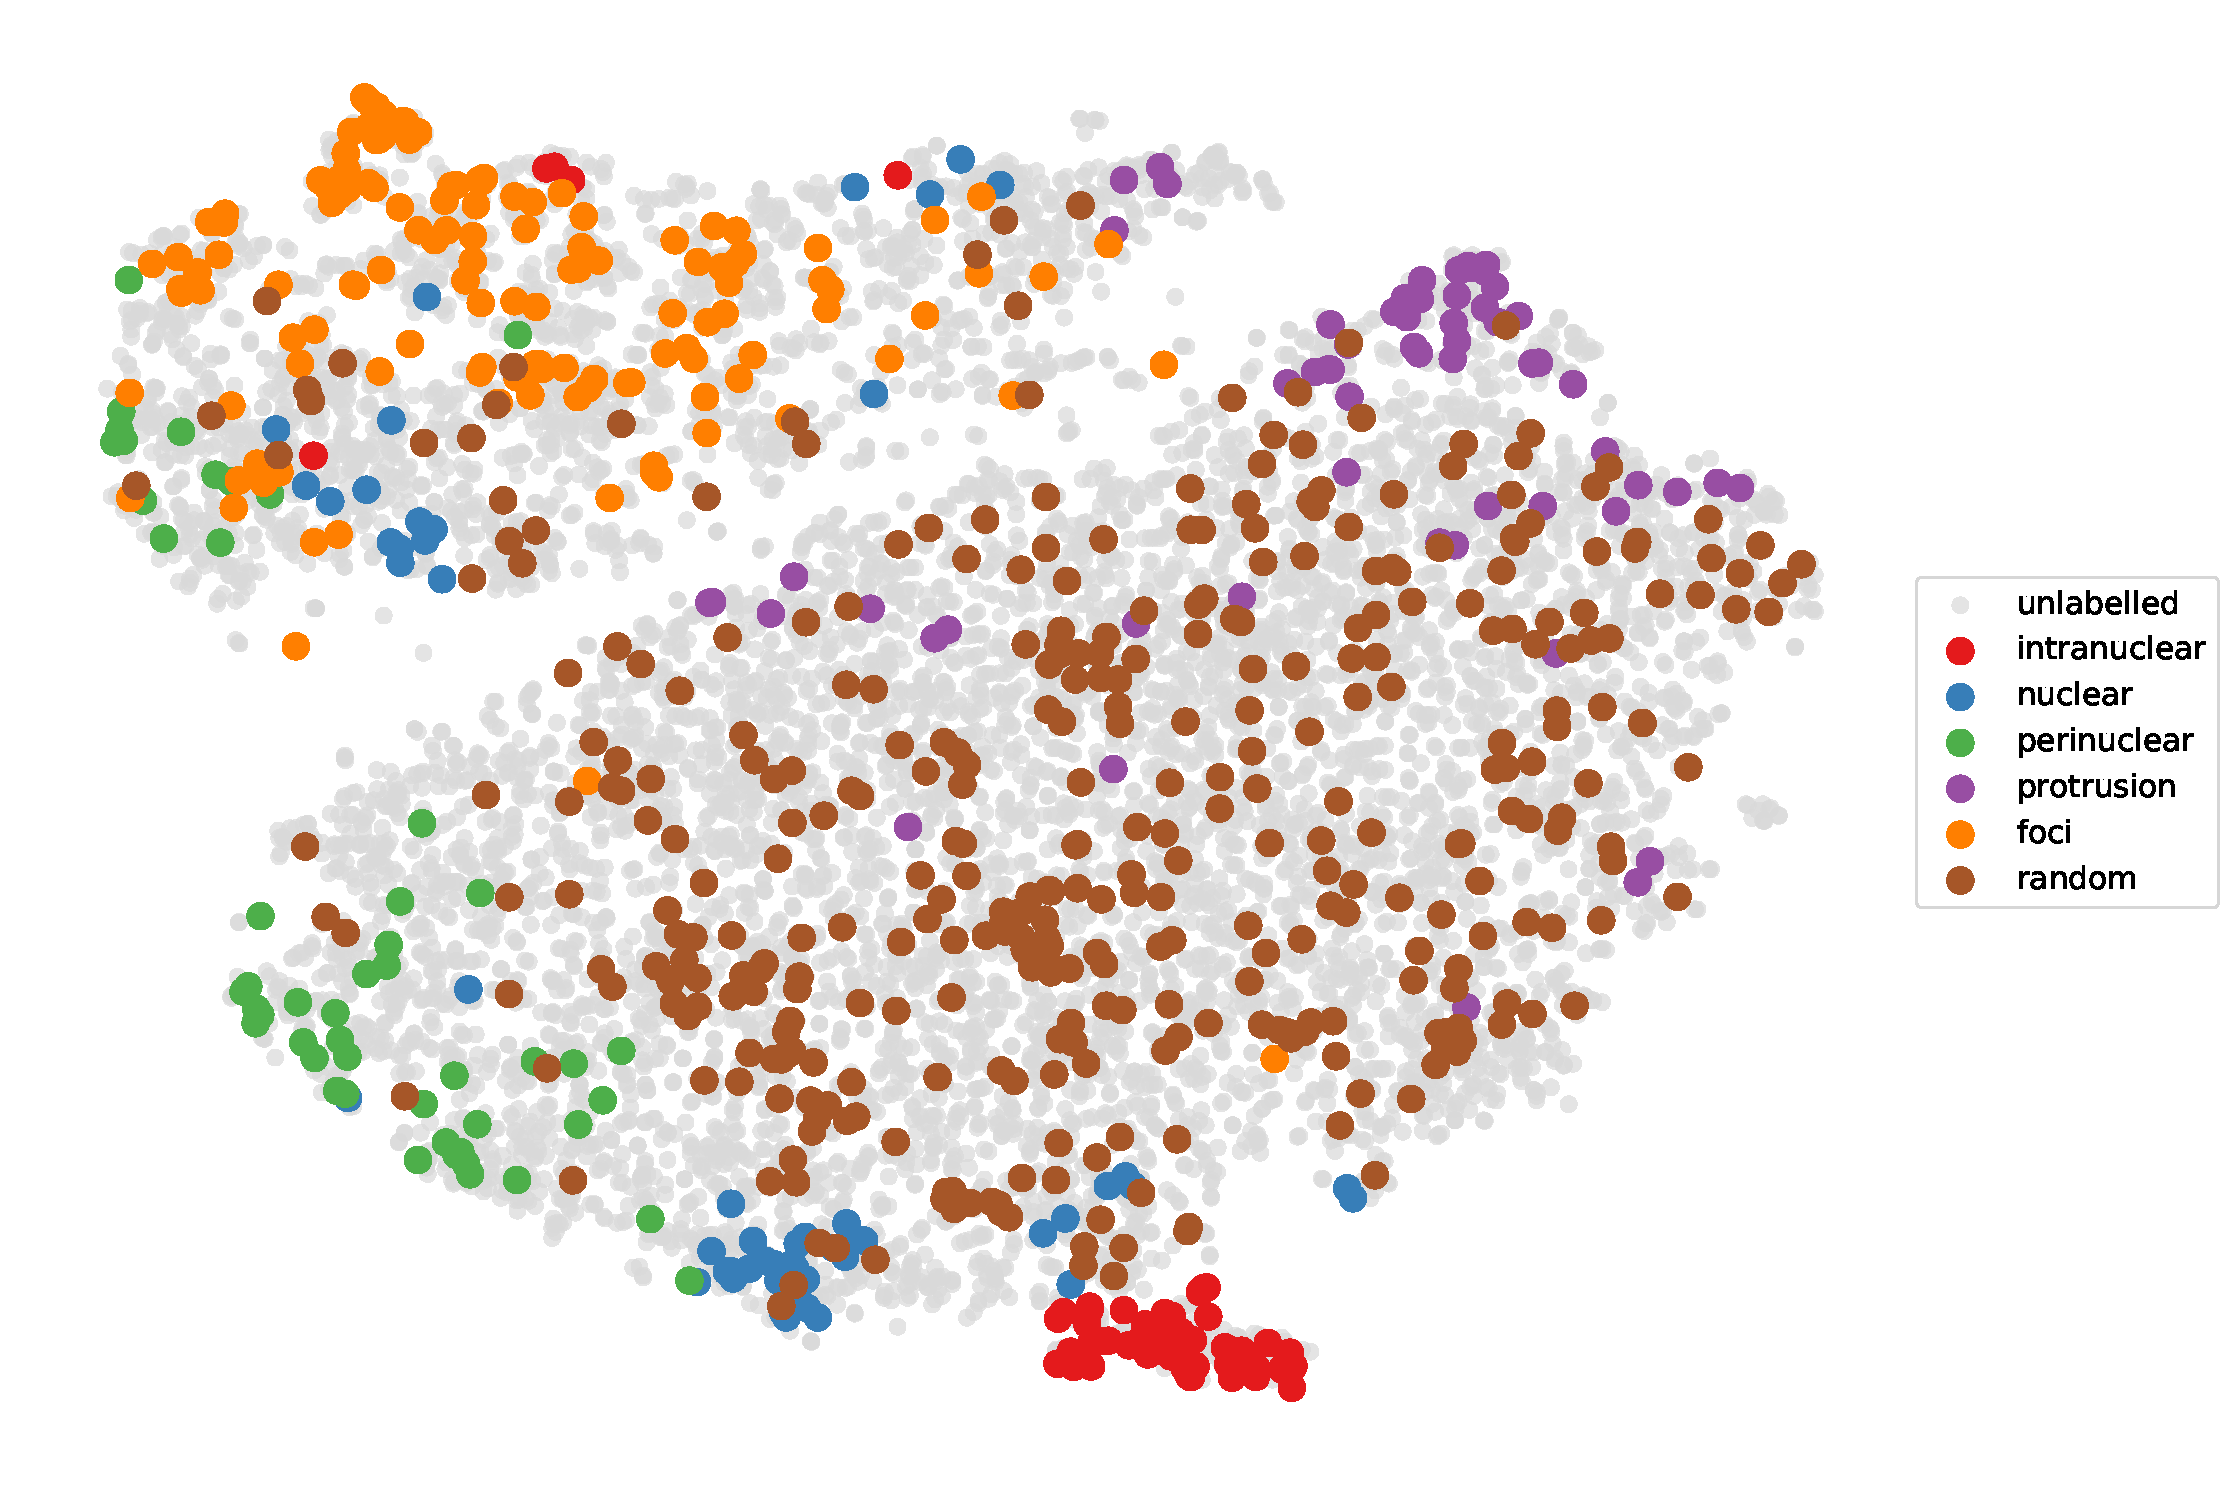
\includegraphics[width=\textwidth]{figures/chapter5/tsne_annotation_legend}
    \caption{t-SNE embedding from~\cite{CHOUAIB_2020}.
	Each point is a cell in the feature space after a t-SNE transformation.
	Manually annotated cells are colored according to their localization pattern.
	Cells that were not annotated or that had multiple patterns are colored in gray}
    \label{fig:tsne_annotation_racha}
\end{figure}

The resulting embedding from the \ac{t-SNE} algorithm can be observed in Figure~\ref{fig:tsne_annotation_racha}.
Cells with different patterns are localized in different regions of the embedded feature space.
Moreover, cells with the same annotations clustered in the same regions whether they correspond to the same gene or not.
With these observations it seems the hand-crafted features capture key information of the localization patterns and summarize well the manual annotations.

Initialized with a PCA transformation, a \ac{t-SNE} algorithm preserves better the global structure, thus allowing more relevant global interpretation.
In particular, we can discriminate on the top a large cluster of cells with a potential foci pattern from the rest of the cell population.
The resulting embedding also seems to polarize between nucleus-related patterns (bottom left) and the cell-related patterns (top right).
This polarization remains even among the subpopulation with potential foci pattern.
Such conclusion validates the design to let a cell being classified with several non-exclusive localization patterns.
Indeed, a foci can be localized in a relevant subcellular compartment.

\subsubsection{Gene aggregated classifications}

% results heatmap (gene level)
% reference to appendix (cell level and consistency unsupervised-supervised)
% biological conclusions

Not surprisingly, a feature space that discriminates well between classes also performs well when fed into a robust random forest classifier.
The \ac{OOB} accuracy score obtained for the different patterns is between 0.93 and 0.99, while a dummy classifier would return a 0.8 accuracy score (the dataset is built with 20\% positive samples).
The intranuclear pattern is the easiest to recognize.
In fact, it could be predicted by just thresholding the proportion of \ac{RNA} inside nucleus (almost all intranuclear cells have more than 80\% of their\ac{RNA}s that localize inside the nucleus).
On the opposite, the nuclear edge and perinuclear patterns are the most difficult to classify due to possible confusion with a random pattern or the lake of annotated cells.

\begin{wraptable}{R}{0.50\textwidth}
	\centering
	\begin{tabular}{| c | c |}
		\hline
		Pattern & Accuracy score\\
		\hline
		Random & -\\
		Foci & 0.95\\
		Intranuclear & 0.99\\
		Nuclear edge & 0.93\\
		Perinuclear & 0.93\\
		Protrusion & 0.94\\
		\hline
		\textit{Dummy classifier} & \textit{0.80}\\
		\hline
	\end{tabular}
	\caption{Random forest accuracy (OOB)}
	\label{table:accuracy_oob}
\end{wraptable}

For each cell, I can compute 5 binary predictions, one per pattern.
If no pattern is detected, cell is classified as random.
In total, I analyze 27 different genes through a population of 9,710 cells, with only one kind of transcript being targeted per cell.
The number of cells identified per gene varies, thus predictions are aggregated at the gene level.
This aggregation also facilitates the validation of biological insights and helps understanding the mechanism at stake for specific group of genes.
For every gene, I compute the proportion of cells displaying each indicated localization pattern.
Results are eventually reported in a heat map~\ref{fig:heatmap_racha_2}, for every gene and pattern.
Importantly, row values does not sum to one because classifiers (and so columns predictions) are  independent.

\begin{wrapfigure}{L}{0.40\textwidth}
	\begin{center}
	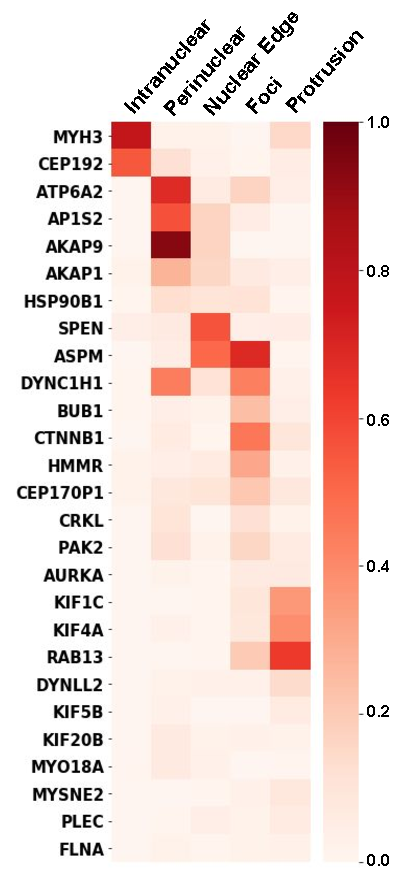
\includegraphics[width=\linewidth]{figures/chapter5/heatmap_racha}
    \caption{Heat map from~\cite{CHOUAIB_2020} with the fraction of cells classified in the indicated pattern}
	\label{fig:heatmap_racha_2}
	\end{center}
\end{wrapfigure}

We manually identify a group of random genes that can be used as a control group: KIF20B, MYO18A, SYNE2 and PLEC.

FLNA transcripts are manually identified with a potential cell edge pattern.
However, such localization is difficult to recognize with the quantitative pipeline, mostly because the pattern is visible in 3D while my cell segmentation, and the spatial features resulting from it, is in 2D.
For these reason we do not study in depth this localization pattern.

Therefore, it is possible, but not shown here, to perform statistical testing over the aggregated predictions.
A Fisher's exact test can measure if the proportion of cells observed with a pattern is significantly greater thant the proportion observed with the control group.

% p_bodies = ["AURKA", "AURKA_puro",
% 			"HMMR", "HMMR_puro",
% 			"CEP170P1", "CRKL", "PAK2"]
% translation_factory = ["DYNC1H1", "DYNC1H1_puro",
% 					   "BUB1", "BUB1_puro",
% 					   "CTNNB1", "CTNNB1_puro"]
% nuclear_edge = ["SPEN", "ASPM", "ASPM_puro"]
% perinuclear = ["ATP6A2", "AP1S2", "AKAP9", "HSP90B1", "AKAP1"]
% intranuclear = ["MYH3", "MYH3_puro", "CEP192"]
% protrusion = ["KIF1C", "KIF1C_puro",
% 			  "KIF4A", "KIF4A_puro",
% 			  "RAB13", "KIF5B", "DYNLL2"]
% random = ["KIF20B", "MYO18A", "MYSNE2", "PLEC", "FLNA"]

%Figure~\ref{fig:tsne_proba_gene}
%Figure~\ref{fig:heatmap_racha_cells}

% racha paper

% results classification & tsne

% To investigate the agreement between unsupervised and supervised analysis and to understand
% the bio- logical signal corresponding to different regions of the t-SNE plot, we
% determined the probabilities of cells to be in a particular pattern, using each of
% the classifier, and plotted this probability on top of the t-SNE representation (Figure 3C).
% Remarkably, cells with a high probability of a given pattern concentrated in the
% same area of the t-SNE plot, thus, providing a direct interpretation of the regions
% with respect to the localization pattern they represent (Fig- ure 3C).
% This also indicated that the assignments of the classifiers were consistent with the manual annotations.


% heatmap

% Finally, we analyzed RNA localization at the gene level. Individ- ual cells were
% assigned to a pattern if the probability given by the random forest classifier for
% that pattern was higher than 0.5. The fractions of cells in each pattern were then
% represented in a heat- map, either directly (Figure S6E) or after filtering out
% cases where the proportion of cells with localized mRNA was not statistically different
% from that of the control random genes (Figure 3D, threshold: p value < 103).
% There was a remarkable agreement between the automated and manual classification.
% Except for FLNA and KIF5B, all the manual annotations were confirmed with high
% degree of statistical significance (p value < 103). FLNA was the only mRNA
% manually annotated as ‘‘cell edge,’’ and we decided not to study it further.
% KIF5B indeed localized weakly in protrusions of HeLa cells (i.e., in a small number of cells),
% although the localization pattern was nicely seen in neuronal cells (Figure S2B).
% The other protrusion mRNAs were statistically different than the controls (p value < 103),
% with 14% (DYNLL2) and up to 62% (RAB13) of the cells classified in that pattern.
% The two genes manually annotated as ‘‘intranu- clear’’ had more than 55% of the cells assigned in that category.
% Likewise, the two ‘‘nuclear edge’’ genes, ASPM and SPEN, had 50% and 55% of cells
% in this category, respectively, while the ‘‘perinuclear’’ genes (AKAP1, AKAP9, AP1S2, ATP6A2, and HSP90B1)
% ranged from 13% (HSP90B1) to 93% (AKAP9). The former value may seem low, but it is nevertheless highly statisti- cally significant (p value of 7.1015).
% Also note that HSP90B1
% mRNAs co-localized with their encoded proteins, providing further evidence that they are localized (see below).
% For the pattern ‘‘foci,’’ the non-P-body genes (ASPM, BUB1, CTNNB1, and DYNC1H1)
% had a high proportion of cells classified in that pattern (24% for BUB1 and up to 69% for ASPM)
% and an average proportion of mRNA in foci varying from 9% (BUB1) to 28% (CTNNB1; Figure S6B).
% In contrast, the mRNAs accumulating in P-bodies had a comparatively smaller fraction of
% cells classi- fied in the ‘‘foci’’ pattern (7% to 31%), as well as a smaller frac- tion
% of the mRNAs in foci (2% to 15%). Note that our estimation of the fraction of mRNA in
% foci correspond to a lower bound because we only counted groups of molecules where each molecule was closer than 350 nm to the group, while foci can be larger.
% Nevertheless, and taking into account our stringent cri- terion, our quantification was in the
% lower range of previously re- ported quantifications of P-body mRNAs (10%–20% of the total mRNAs; Pillai et al., 2005; Hubstenberger et al., 2017).
% When comparing individual cells, the quantifications indicated that RNA localization
% can be highly variable even for the same mRNA. For instance, the fraction of CTNNB1 mRNA
% in foci varied from 0% to more than 60%. To analyze this phenomenon in more details,
% we plotted the cells of each single gene on t-SNE plots (Figure S7), and we also
% generated heatmaps depicting the probabilities of the different patterns for all the individual cells (Figures 3E and S7).
% This provided a very detailed view of RNA localization at the level of single cells.
% It confirmed the intercel- lular variability of RNA localization as cells of a given
% gene were dispersed of the t-SNE plot, although an accumulation in the expected area of the plot was visible (Figure S7).
% Likewise, the pattern probabilities varied greatly from cell to cell (Figure S7).
% It was also apparent that a large number of cells had several pat- terns simultaneously.
% In particular, many DYNC1H1 cells were classified as both ‘‘perinuclear’’ and ‘‘foci,’’
% and many ASPM cells were both ‘‘nuclear edge’’ and ‘‘foci’’ (in agreement with the manual annotations).
% Likewise, MYH3 cells were frequently ‘‘intranuclear’’ and ‘‘protrusion.’’
% In conclusion, this quantitative analysis corroborated the manual annotations and revealed a high degree of heterogeneity of RNA localization across different cells.
% This heterogeneity is a general phenomenon since it is seen with nearly all the genes analyzed here.


%%%%%%%%%%%%%%%%%%%%%%%%%%%%%%%%%%%%%%%%%%%%%%%%%%%%%%%%%%%%%%%%%%%%%%%%%%%%%%
%%%%%%%%%%%%%%%%%%%%%%%%%%%%%%%%%%%%%%%%%%%%%%%%%%%%%%%%%%%%%%%%%%%%%%%%%%%%%%
%%%%%%%%%%%%%%%%%%%%%%%%%%%%%%%%%%%%%%%%%%%%%%%%%%%%%%%%%%%%%%%%%%%%%%%%%%%%%%

\section{Translation factories}
\label{sec:translation_factories}

A second important results unveiled in~\cite{CHOUAIB_2020} is the identification and the quantification of a cluster-based localization pattern we name \emph{translation factory}.

\subsection{Introduction}
\label{subsec:introduction_translation_factories}

\begin{center}
	\textit{(To be completed)}
\end{center}

% paper FQ2

% In Chouaib et al. (2020), we performed a high-content screen in HeLa cells and analyzed 10,000 segmented cells.
% FISH-quant v2 was used for spot detection, cell segmenta- tion and the computation of localization features
% that al- lowed us to apply supervised and unsupervised machine learning to identify localization patterns and
% classify single cells into predefined pattern classes. We observed several distinct mRNA localization patterns,
% including RNA accu- mulating (i) in foci, (ii) in cytoplasmic protrusions, (iii) in the perinuclear area
% (which could be subdivided in endo- somal, RE, Golgi and centrosome associate), (iv) forming a rim at the nuclear edge, or (v) inside the nucleus (Fig. 2).
% Interestingly, automated classification done on a single-cell level revealed a high degree of
% cell-to-cell het- erogeneity in RNA localization, with 10% to 80% of the cells displaying the
% expected pattern depending on the RNA (Fig. 5A). In addition, for each pattern, only a fraction of
% the mRNA appeared to localize, revealing a high degree of plasticity in RNA localization mechanisms.
% This appears to be specific to cell lines as RNA localization in embryos is usually much more stereotyped.
% We also quantified how translation inhibition affected RNA localization and found that most mRNAs localize in a
% translation-dependent man- ner, which is unexpected (Fig. 5B). This also enabled us to discover translation factories,
% small cytoplasmic structures where specific mRNAs accumulate to be translated.

\begin{figure}[h]
    \centering
    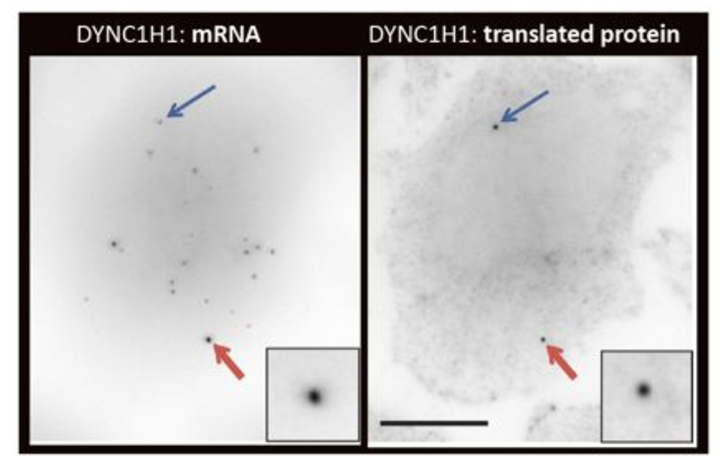
\includegraphics[width=\textwidth]{figures/chapter5/translation_factory}
    \caption{Colocalization between the DYNC1H1 transcript and its nascent protein, from~\cite{pichon_visualization_2016}.
	Transcripts and proteins are targeted with smFISH probes (\textit{Left}) and SunTag (\textit{Right}) respectively.
	\textit{Scale bar} is 10μm}
    \label{fig:translation_factory}
\end{figure}

\subsection{Materials and methods}
\label{subsec:materials_translation_factories}

% paper Racha

% To measure the degree of spatial overlap between mRNA (by smFISH) and protein
% (by the GFP fluorescence), we calculated an enrichment ratio. Cells and nuclei
% were outlined manually in 2D based on the GFP and DAPI image, respectively.
% The subsequent analysis was restricted to the cytoplasm. FISH-quant was used
% to detect mRNAs in 3D and each cell was post-processed separately.
% First, we calculated the median pixel intensity in the GFP image at the identified RNA positions.
% Second, we estimated a normalization factor as the median GFP intensity of the outlined cytoplasm within the z-range of the detected mRNAs.
% The enrichment ratio was then estimated as the ratio of the median GFP intensity at the RNA positions divided by the mean cytoplasmic GFP intensity.

\subsubsection{Puromycin drug}

\subsubsection{Cluster detection}

% distinct  from the dense decomposition

\subsection{Results}
\label{subsec:results_translation_factories}

\begin{figure}[h]
    \centering
    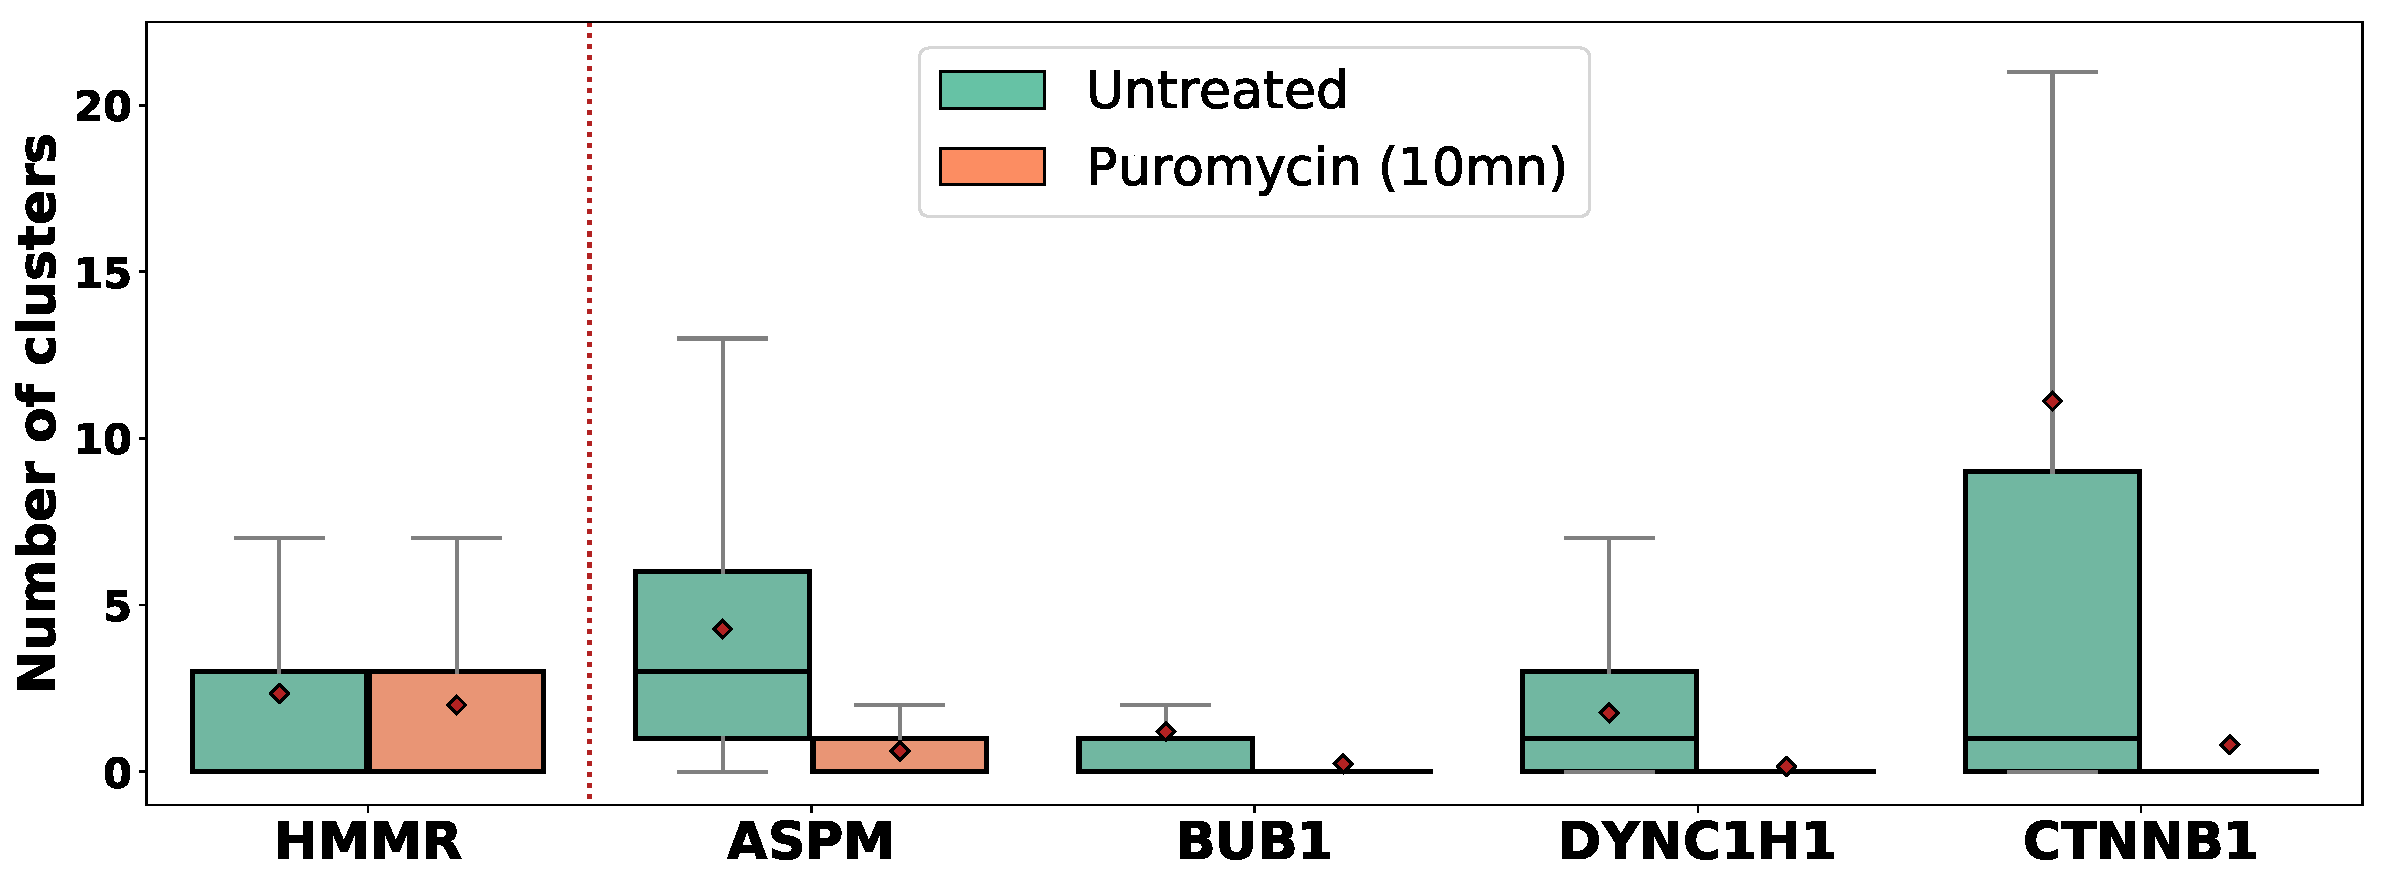
\includegraphics[width=\textwidth]{figures/chapter5/plot_puromycin}
    \caption{Impact of treatment with translational inhibitor puromycin on the number of detected RNA clusters}
    \label{fig:plot_puromycin}
\end{figure}

% paper fq2
% HMMR shows a similar number of clusters, while all other genes have significantly fewer, indicating an implication of translation in cluster formation.

%%%%%%%%%%%%%%%%%%%%%%%%%%%%%%%%%%%%%%%%%%%%%%%%%%%%%%%%%%%%%%%%%%%%%%%%%%%%%%
%%%%%%%%%%%%%%%%%%%%%%%%%%%%%%%%%%%%%%%%%%%%%%%%%%%%%%%%%%%%%%%%%%%%%%%%%%%%%%
%%%%%%%%%%%%%%%%%%%%%%%%%%%%%%%%%%%%%%%%%%%%%%%%%%%%%%%%%%%%%%%%%%%%%%%%%%%%%%

\section{Centrosomal pattern}
\label{sec:centrosomal}

\begin{center}
	\textit{(To be completed)}
\end{center}

\subsection{Introduction}
\label{subsec:introduction_centrosomal}

\begin{figure}[h]
    \centering
    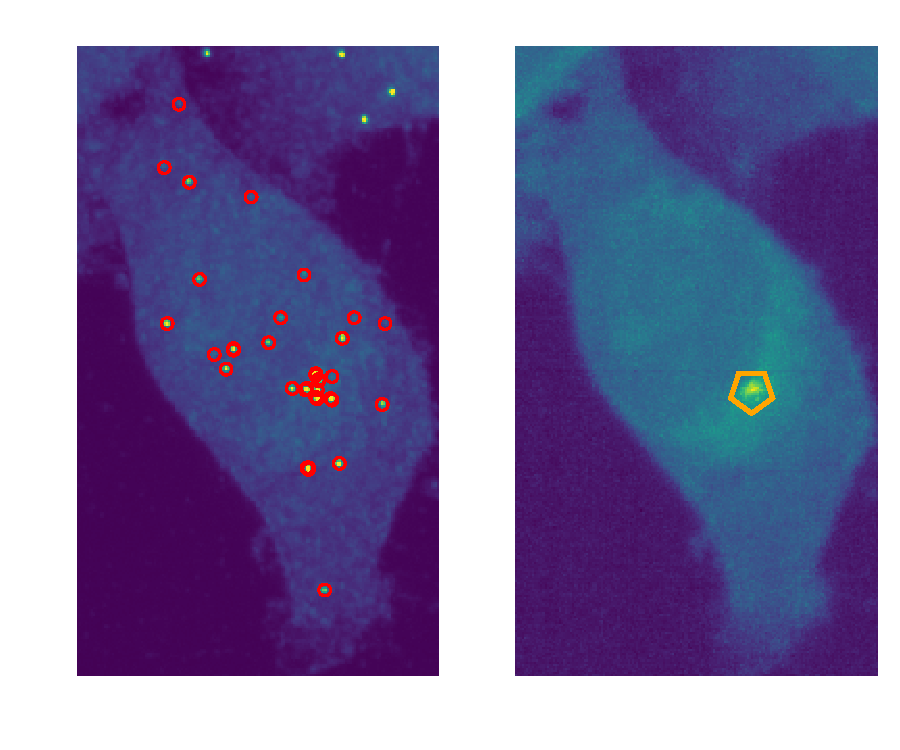
\includegraphics[width=\textwidth]{figures/chapter5/centrosomes}
    \caption{Contrasted image with detected RNAs on a smFISH channel (\textit{left}) and detected centrosome on a GFP channel (\textit{right}).
	Targeted transcript is BICD2.
	Plot build with \emph{bigfish}}
    \label{fig:centrosomes}
\end{figure}

\subsection{Materials and methods}
\label{subsec:materials_centrosomal}

\subsubsection{Experimental data}

\begin{figure}[h]
    \centering
    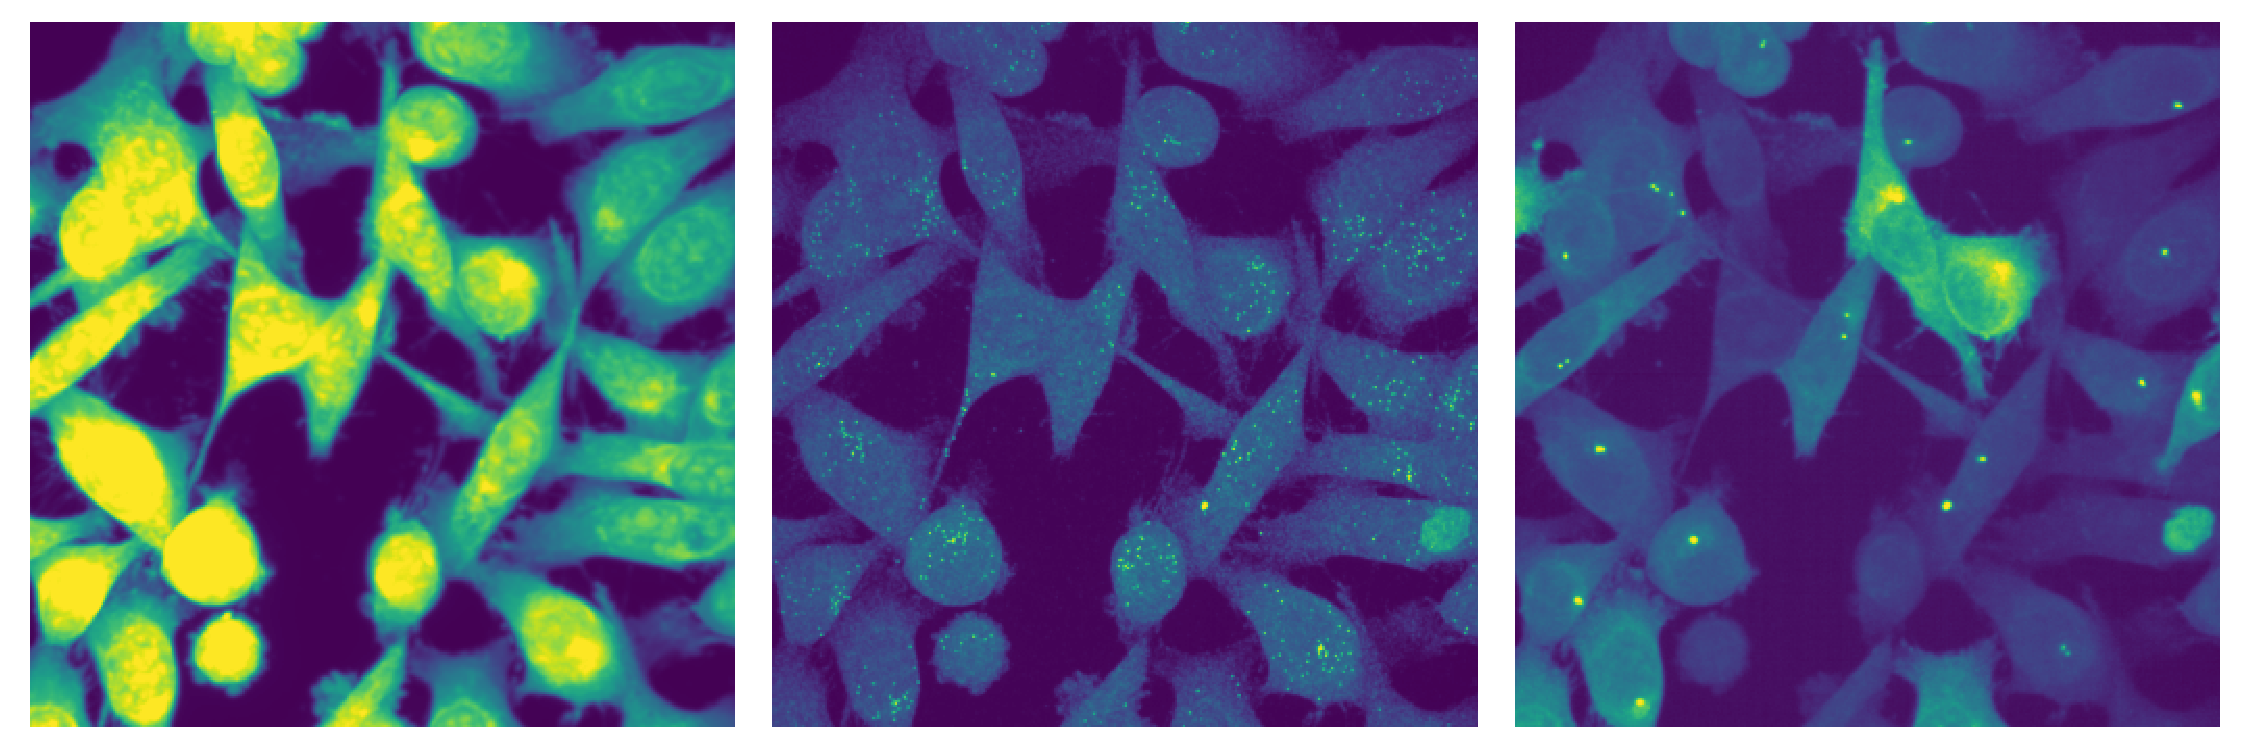
\includegraphics[width=\textwidth]{figures/chapter5/FoV_BICD2}
    \caption{Contrasted image with CellMask\textsuperscript{\texttrademark} (\textit{left}), smFISH (\textit{center}) and GFP (\textit{right}) channels.
	Targeted transcript is BICD2.
	Images are projected in 2D.
	Plot build with \emph{bigfish}}
    \label{fig:fov_adham}
\end{figure}

\subsubsection{Centrosome detection}

\subsubsection{Cell and nucleus segmentation}

\subsection{Results}
\label{subsec:results_centrosomal}

\subsubsection{Centrosomal mRNAs}

\begin{figure}[h]
    \centering
    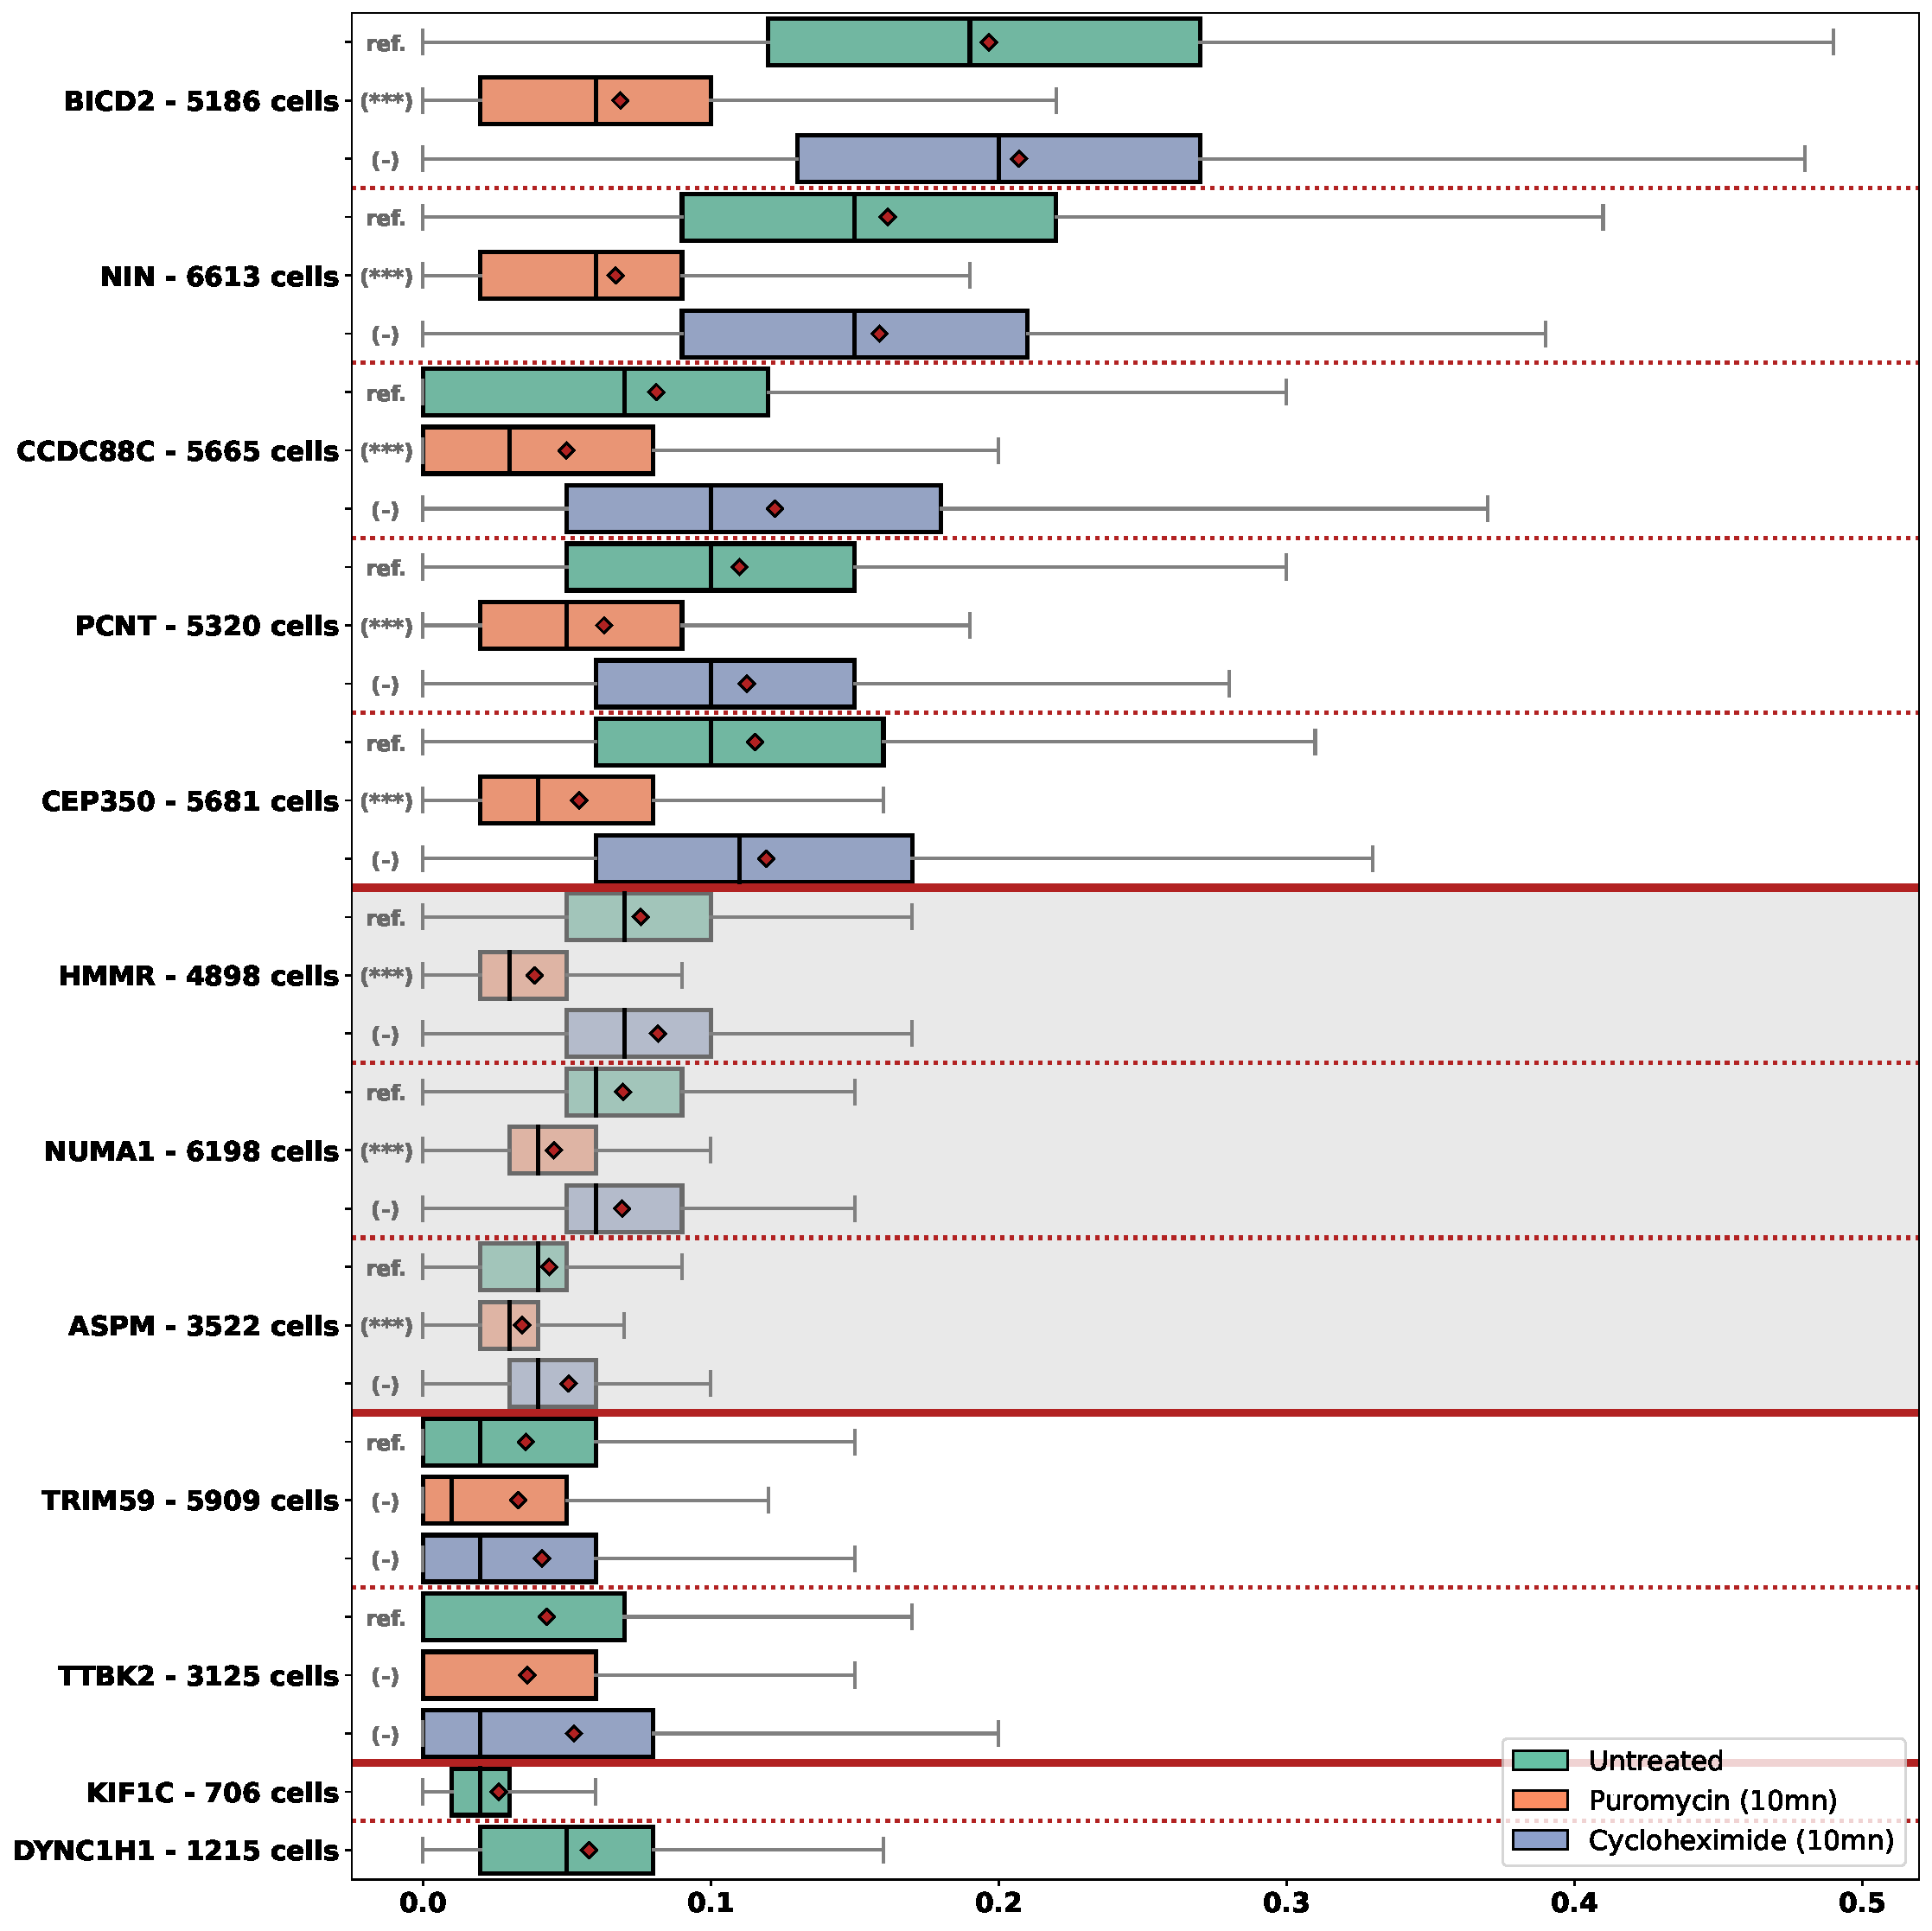
\includegraphics[width=\textwidth]{figures/chapter5/plot_rna_centrosome}
    \caption{Box plot with the proportion of centrosomal mRNAs in cells, for different genes and treatments.
	The \textit{whiskers} equal 1.5 the interquartile range.
	HMMR (in \textit{gray}) is an endogenous centrosomal mRNAs, the rest are BAC-transcribed mRNAs.
	A one-sided Welch’s t test is used to evaluate significance}
    \label{fig:plot_rna_centrosome}
\end{figure}

% Box plots depicting the proportion of centrosomal mRNAs in cells (interphase and mitotic),
% for the indicated mRNAs and cell treatments. Values were computed for each cell and the
% number of cells analyzed is indicated. The distribution of the values is depicted in the boxed plot.
% The colored area corresponds to the second and third quartiles, the mean to the black vertical bar,
% and the median to the red diamond. The whiskers equal 1.5 the interquartile range.
% The right graph represents endogenous centrosomal mRNAs, while the left one represents
% BAC-transcribed mRNAs. Significance was evaluated with a one-sided Welch’s t test.
% ***: null hypothesis rejected with a 0.1% significance level, and -: null hypothesis not rejected.

\subsubsection{Influence of mitosis}

%%%%%%%%%%%%%%%%%%%%%%%%%%%%%%%%%%%%%%%%%%%%%%%%%%%%%%%%%%%%%%%%%%%%%%%%%%%%%%
%%%%%%%%%%%%%%%%%%%%%%%%%%%%%%%%%%%%%%%%%%%%%%%%%%%%%%%%%%%%%%%%%%%%%%%%%%%%%%
%%%%%%%%%%%%%%%%%%%%%%%%%%%%%%%%%%%%%%%%%%%%%%%%%%%%%%%%%%%%%%%%%%%%%%%%%%%%%%

\section{Protrusion pattern}
\label{sec:protrusion}

\begin{center}
	\textit{(To be completed)}
\end{center}

\subsection{Introduction}
\label{subsec:introduction_protrusion}

\subsection{Materials and methods}
\label{subsec:materials_protrusion}

\subsection{Results}
\label{subsec:results_protrusion}

\section{Exploring large scale dataset}
\label{sec:exploration}

\begin{center}
	\textit{(To be completed)}
\end{center}

%~\cite{lecuyer_global_2007}

%To address this point, we developed and employed a high-resolution fluorescent
%in situ hybridization procedure to comprehensively evaluate mRNA localization
%dynamics during early Drosophila embryogenesis. Surprisingly, of the 3370 genes
%analyzed, 71\% of those expressed encode subcellularly localized mRNAs.
%Dozens of new and striking localization patterns were observed, implying an
%equivalent variety of localization mechanisms. Tight correlations between mRNA
%distribution and subsequent protein localization and function, indicate major
%roles for mRNA localization in nucleating localized cellular machineries.

%Computational Analysis The annotation data was converted into a binary matrix,
%containing genes on one axis and localization terms on the other, where the presence
%of a localization feature for a given gene was indicated numerically as ‘‘1,’’
%while lack of a feature was annotated as ‘‘0.’’ This matrix was then used for GO
%term enrichment analysis. Functional GO annotations for all genes were downloaded
%from Flybase (http://flybase.bio. indiana.edu/genes/lk/function/). Annotations
%were up-propagated using the GO hierarchy (Ashburner et al., 2000), and calculations
%were restricted to genes that were both GO annotated and analyzed in this study
%(1651 genes). The hypergeometric distribution was used to calculate probabilities
%of overlap between each localization category against all GO categories containing
%three or more genes. The Benjamini-Hochberg procedure (Benjamini and Hochberg, 1995)
%was used to control for multiple testing by computing a P-value threshold
%corresponding to a false discovery rate (FDR) of 0.25. Transcript subgroups
%were also analyzed independently for GO term enrichments using EASE (Hosack et al., 2003).
%EASE scores of less that 0.05 were considered significant, as reported previously (Tadros et al., 2007a).

\section{Conclusion}
\label{sec:conclusion_chapter5}

\begin{center}
	\textit{(To be completed)}
\end{center}